
\begin{frame}
  {Übersicht}
  \begin{itemize}[<+->]
    \item Deskriptive Statistik als \alert{Aggregation von Daten}
      \Halbzeile
    \item Verteilungen in Stichproben und Grundgesamtheiten:
      \begin{itemize}
	\item Zentralmaße
	\item Streuung (Varianz)
      \end{itemize}
    \item \orongsch{Theoretische vs.\ empirische Verteilungen}
      \Halbzeile
    \item \alert{Konfidenzintervalle} | Genauigkeiten von Schätzungen?
  \end{itemize}
\end{frame}

\begin{frame}
  {Literatur}
  \begin{itemize}
    \item Google, Stackoverflow usw.
      \Zeile
    \item \citet{GravetterWallnau2007}\\
      Achtung! \orongsch{Vermittelt eine falsche Philosophie bei Anwendung der Tests!}
      \Halbzeile
    \item \citet{Bortz2010}
  \end{itemize}
\end{frame}

\section{Motivation}

\begin{frame}
  {Zweck der deskriptiven Statistik}
  \begin{itemize}[<+->]
    \item Mit unbewaffnetem Auge auf Daten zu blicken, ist meistens zwecklos.
      \Halbzeile
    \item In Zahlen sehen Menschen nur schlecht Tendenzen und Zusammanhänge.
      \Zeile
    \item Deskriptive Statistik
      \begin{itemize}[<+->]
        \item \alert{Zusammenfassen}
        \item \alert{Gruppieren}
        \item \alert{Visualisieren}
      \end{itemize}
  \end{itemize}
\end{frame}


\begin{frame}
  {Was will man wissen?}
  \begin{itemize}[<+->]
    \item Definition der Grundgesamtheit
      \Halbzeile
    \item \alert{Stichprobengröße ($n$)}
      \begin{itemize}[<+->]
        \item 200 Sätze aus dem Korpus
        \item 1.000 Reaktionen (von 50 Probanden) im Experiment
        \item Was sind die elementaren gemessenen Datenpunkte?
      \end{itemize}
      \Halbzeile
    \item Stichprobenmethode
      \begin{itemize}[<+->]
        \item \alert{Zufallsstichprobe} | Nachweis der uniformen Zufälligkeit
        \item \alert{Quotenstichprobe} | Stratifzierung und Begründung
      \end{itemize}
  \end{itemize}
\end{frame}


\section{Skalenniveau}

\begin{frame}
  {Messvariablen und Skalenniveaus}
  \begin{itemize}[<+->]
    \item \alert{dichotom\slash binär} | \gruen{Menge $\{A, B\}$} | zwei disjunkte Kategorien\\
      \grau{männlich, weiblich ; Präteritum, Perfekt}
      \Viertelzeile
    \item \alert{nominal\slash kategorial} | \gruen{Menge $\{A, B, ..\}$} | disjunkte Kategorien\\
      \grau{Parteizugehörigkeit ; NP, AP, VP}
      \Viertelzeile
    \item \alert{ordinal} | \gruen{Tupel $\langle A, B, ..\rangle$, \rot{nicht} $\mathbb{N}$ oder $\mathbb{Z}$} | disjunkte Kategorien mit Rang\\
      \grau{Schulnoten ; 5- oder 7-Punkt-Skalen für Akzeptabilität}\\
      \Viertelzeile
    \item \alert{Verhältnis} | \gruen{$+\mathbb{Q}_0$} | geordnete Werte mit Nullpunkt\\
      \grau{Temperatur in Kelvin ; Lesezeiten}
      \Viertelzeile
    \item \alert{Intervall} | \gruen{$\mathbb{Q}$} | Wie Verhältnis, aber ohne Nullpunkt\\
      \grau{Temperatur in Celsius}
      \Zeile
    \item \rot{Zähldaten} | \rot{Keine} beobachtbaren Variablen, sondern\\
      Aggregation von dichtotomen, nominalen oder ordinalen Variablen\\
  \end{itemize}
\end{frame}

\begin{frame}
  {Intervalle vs.\ Verhältnisse}
  \begin{itemize}[<+->]
    \item \alert{Verhältnisskala} | Größe von Menschen in cm
      \begin{itemize}[<+->]
	\item $200 cm = 2 \times 100 cm$ usw.
	\item Keine Messung unter $0 cm$ 
      \end{itemize}
      \Zeile
    \item \alert{Intervallskala} | Dasselbe als \alert{Abweichung vom Mittel}
      \begin{itemize}[<+->]
	\item $4 cm = 2 \times 2 cm$ usw.
        \item \orongsch{$184 cm \neq 2 \times 182 cm$}
	\item Negative Messungen möglich
      \end{itemize}
  \end{itemize}
\end{frame}

\begin{frame}
  {Relevanz der Skalenniveaus}
  \begin{itemize}[<+->]
    \item Bestimmung \alert{zulässiger mathematischer Operationen}
      \Halbzeile
    \item \alert{Deskriptive Statistiken} je nach Skalenniveau
      \Halbzeile
    \item Zulässigkeit von \alert{inferenzstatistischen Tests} je nach Skalenniveau
  \end{itemize}
\end{frame}


\section{Zentraltendenz}

\begin{frame}
  {Zentraltendenz I}
  \alert{Modus} | Der \alert{häufigste Wert} | \orongsch{Alle Skalenniveaus}\\
  \Zeile
  \begin{center}
    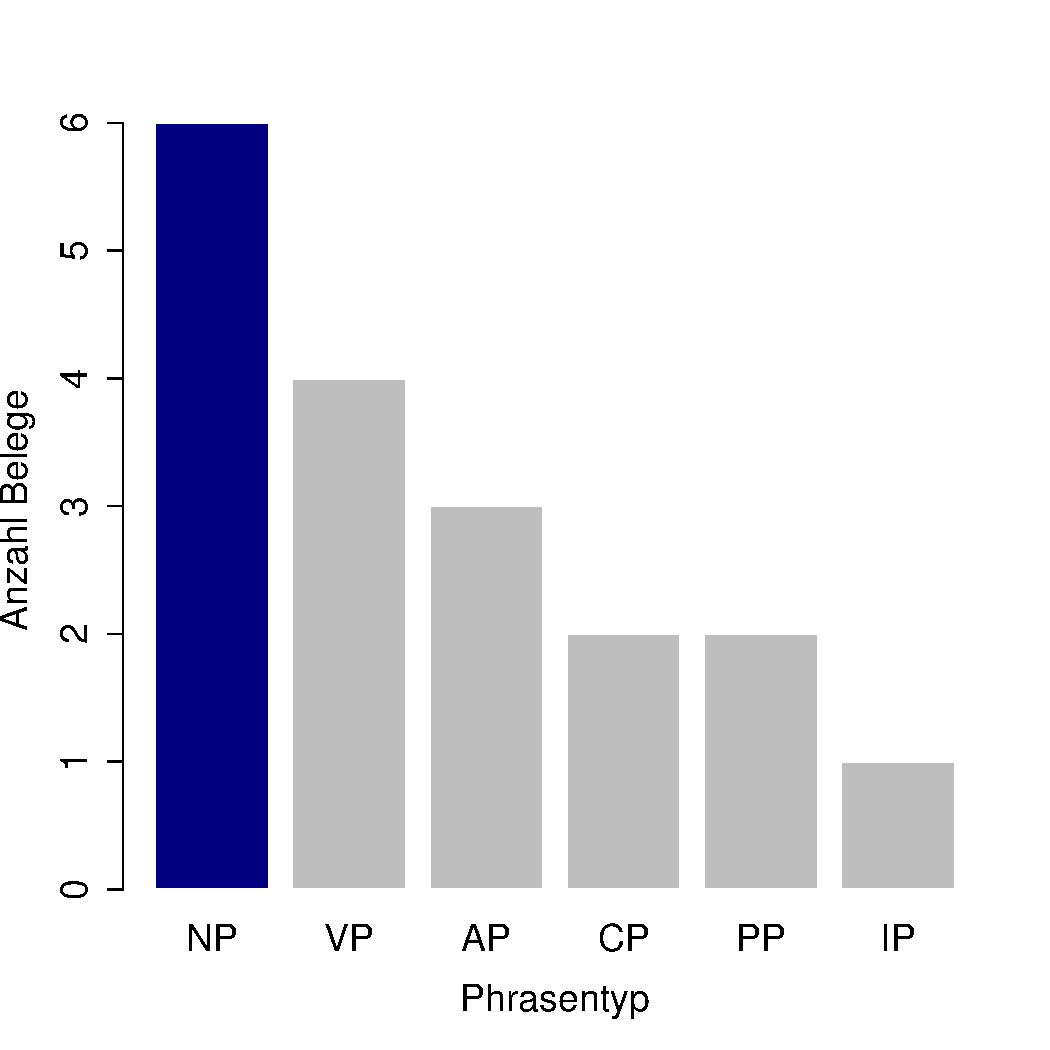
\includegraphics[height=0.6\textheight]{RVorlesung/mode}
  \end{center}
\end{frame}

\begin{frame}
  {Zentraltendenz II}
  \alert{Median} | \alert{Mitte der sortierten Stichprobe} | \orongsch{ab Ordinalskala}\\
  \Zeile
  \begin{center}
    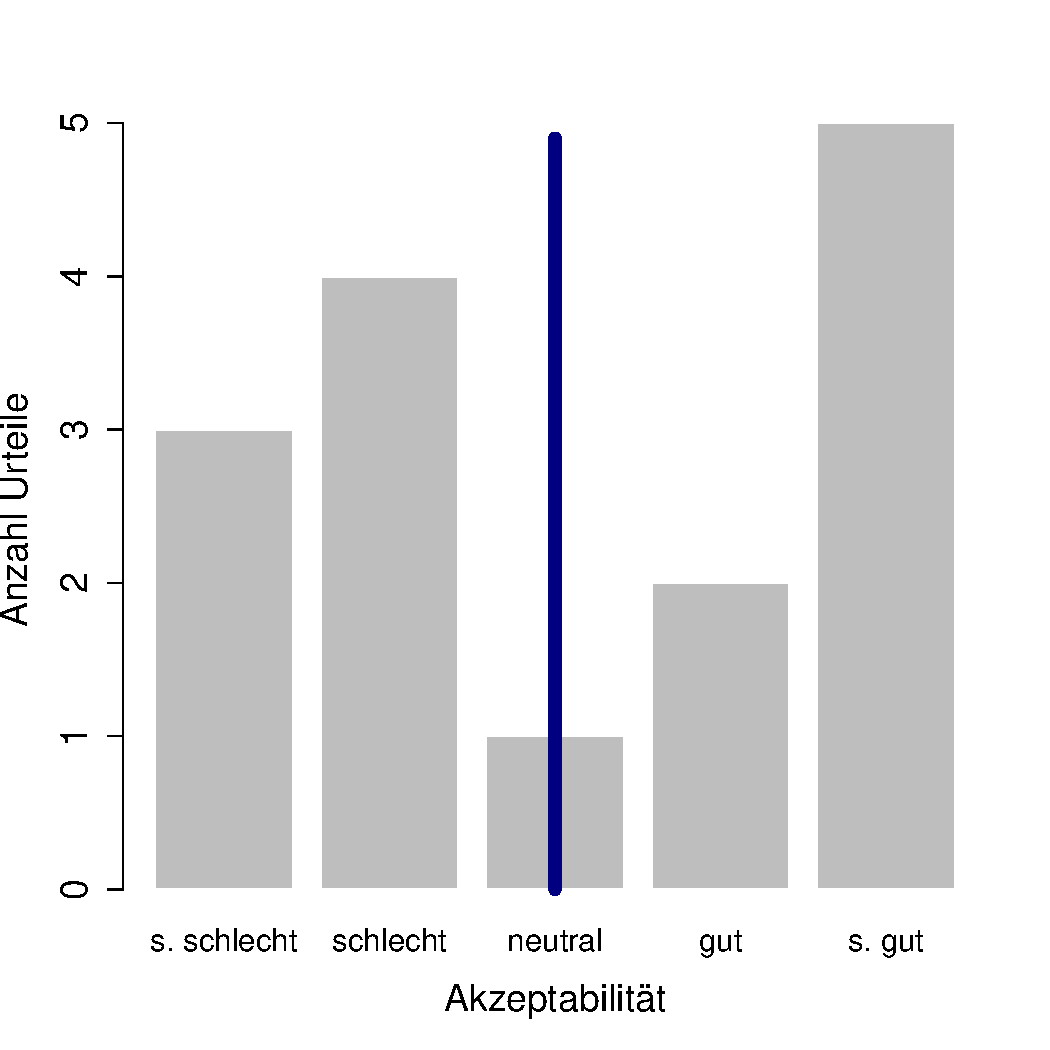
\includegraphics[height=0.6\textheight]{RVorlesung/median}
  \end{center}
  \Zeile
  \grau{\footnotesize Numerische Messungen | Verschiedene Interpolationsmethoden\\
    \url{https://en.wikipedia.org/wiki/Quantile\#Estimating_quantiles_from_a_sample}}
\end{frame}

\begin{frame}
  {Median bestimmen | Stichprobe}
  \centering 
  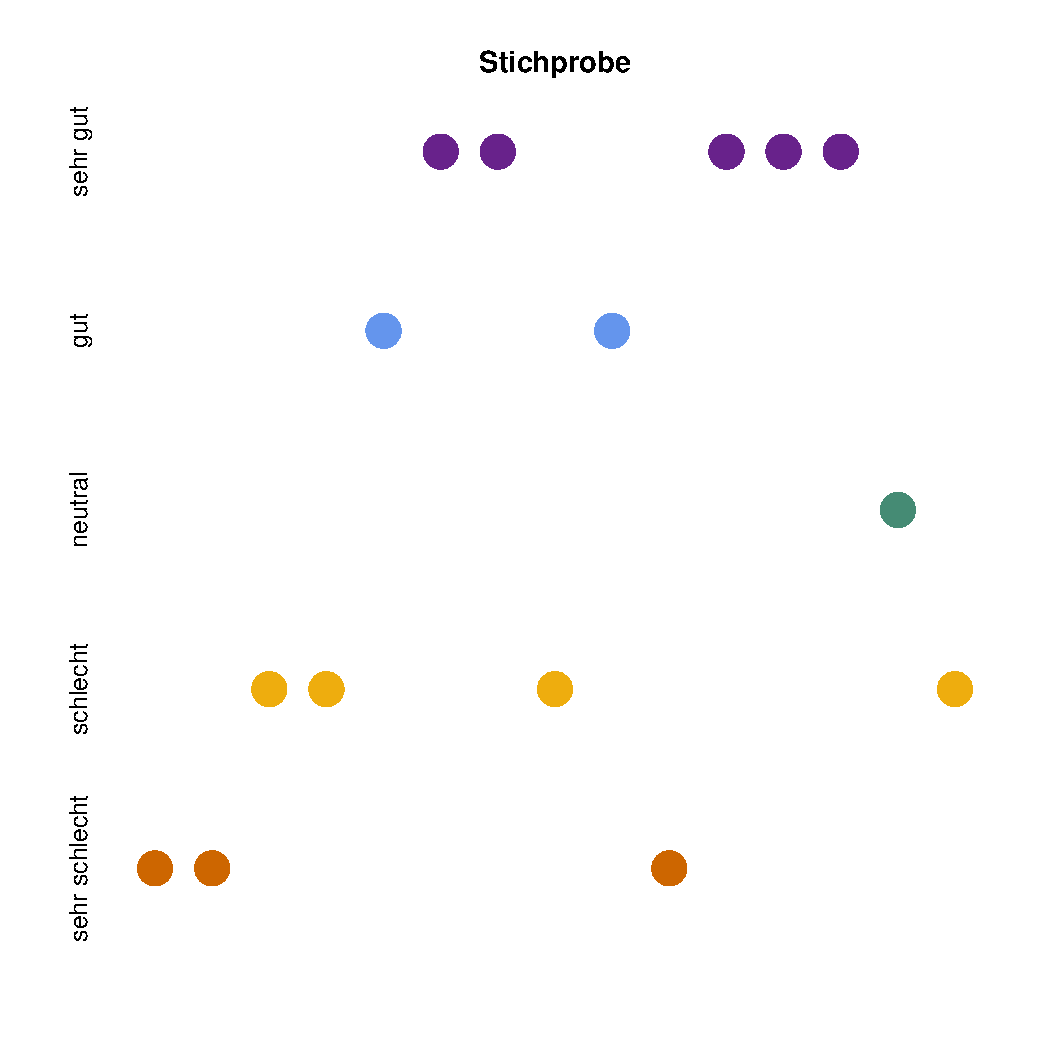
\includegraphics[height=0.9\textheight]{RVorlesung/median1a}
\end{frame}

\begin{frame}
  {Median bestimmen | Sortierte Stichprobe}
  \centering 
  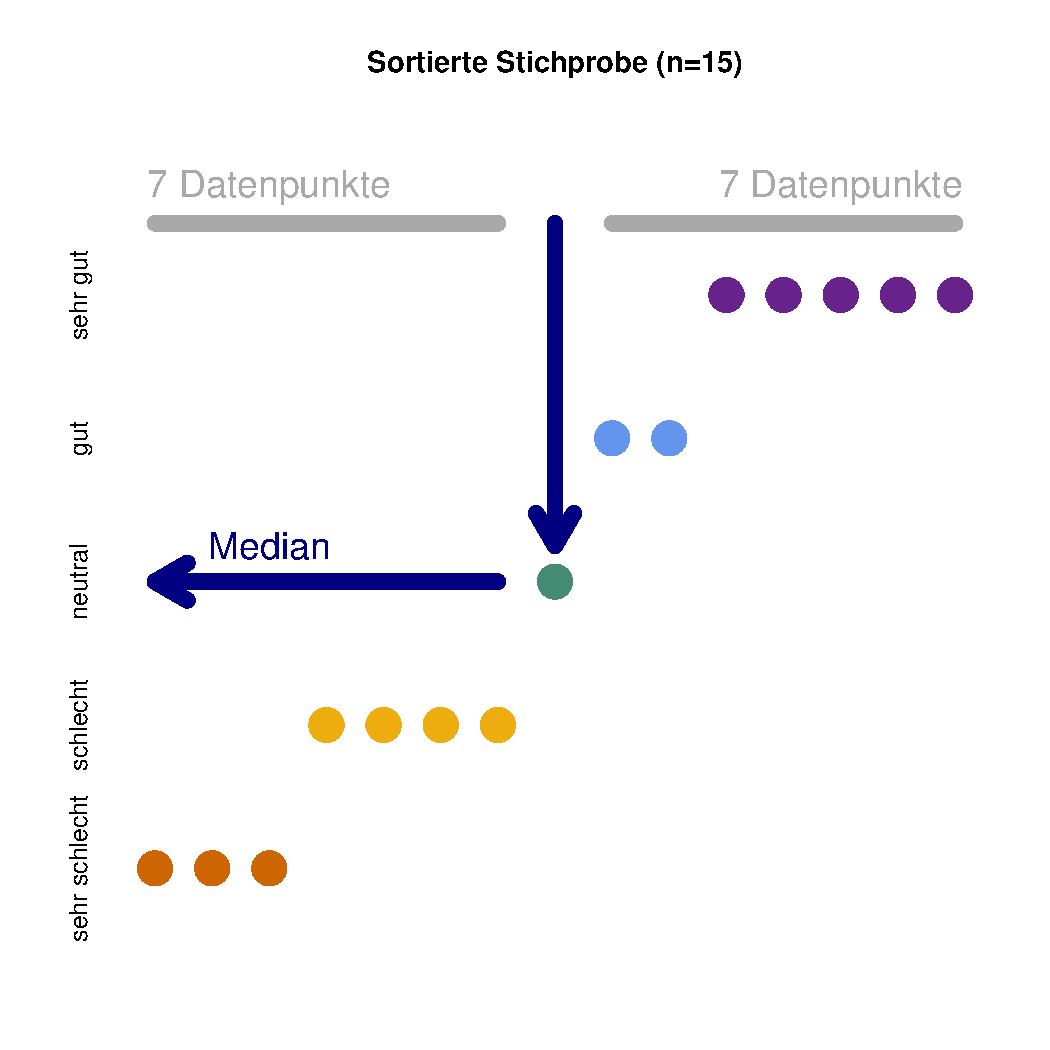
\includegraphics[height=0.9\textheight]{RVorlesung/median1b}
\end{frame}

\begin{frame}
  {Median bestimmen | Verzerrtere sortierte Stichprobe}
  \centering 
  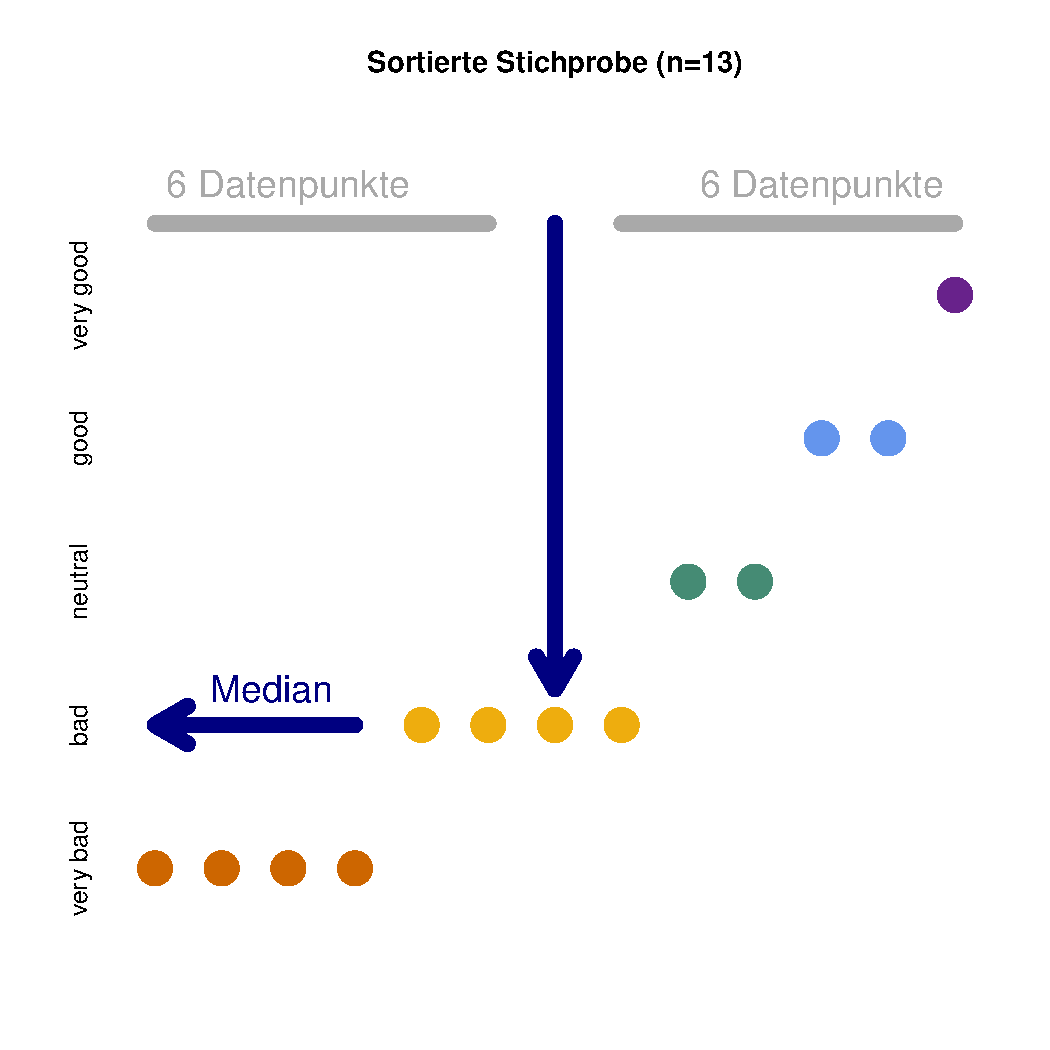
\includegraphics[height=0.9\textheight]{RVorlesung/median2}
\end{frame}

\begin{frame}
  {Zentraltendenz III}
  \alert{Arithmetisches Mittel} $\bar{x}$ | Summe aller Werte geteilt durch $n$ | \orongsch{ab Intervallskala}\\
  \Zeile
  \begin{multicols}{2}
    \centering 
    \hspace{0em}\\
    \vspace{0.1\textheight}
    $\bar{x}=\frac{\sum\limits_{i=1}^{n}x_i}{n}$
    \newpage
    \raggedright
    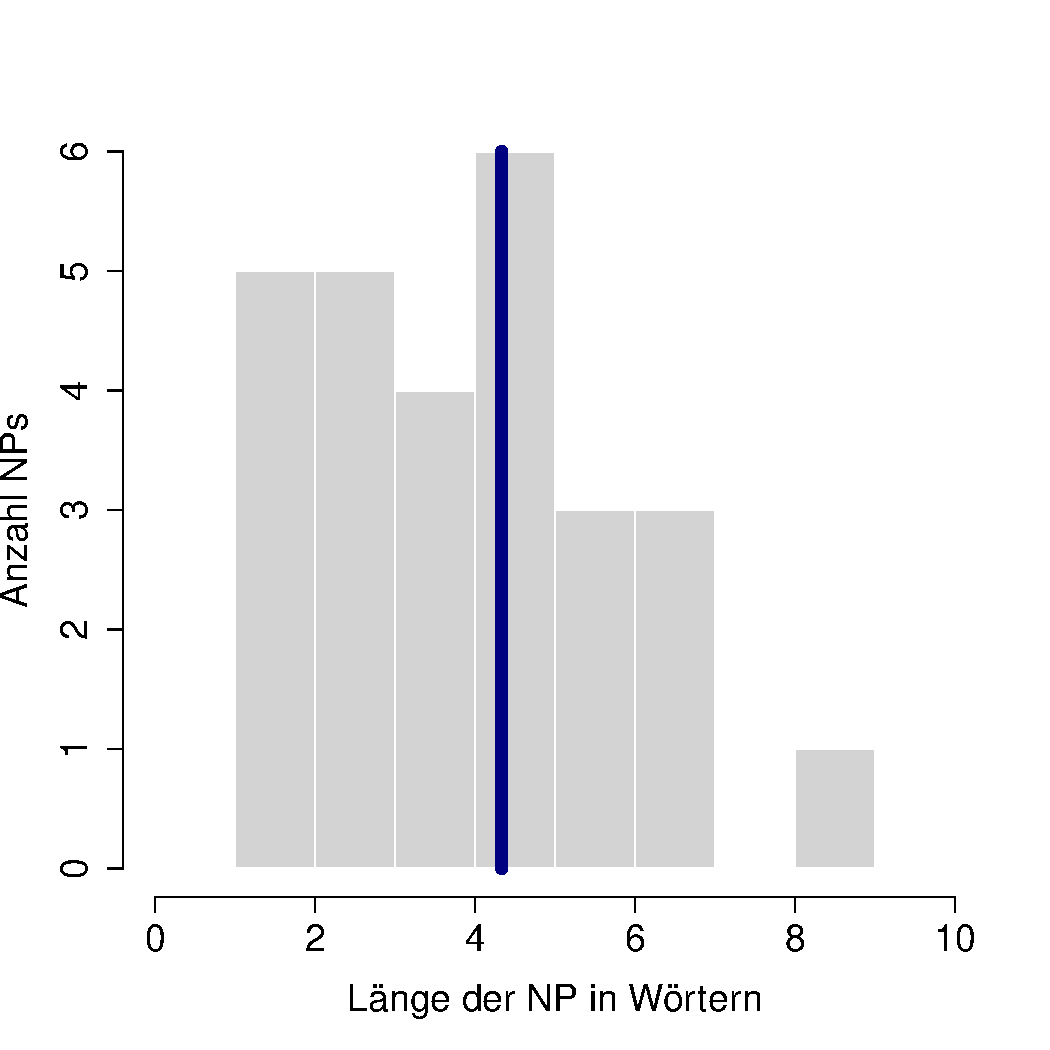
\includegraphics[height=0.6\textheight]{RVorlesung/mean}
  \end{multicols}
\end{frame}



\section{Empirische Verteilungen und Dispersion}

\begin{frame}
  {Warum sind Dispersionsmaße wichtig?}
  \alert{Dispersion} | Streuung der Daten\\
  \Zeile
  \begin{itemize}[<+->]
    \item \alert{Zentraltendenz} | Orientierung über Tendenzen der Stichprobe
     \Zeile 
    \item \alert{Ein Maß für Zentraltendenz} für \orongsch{beliebig viele Verteilungsformen}
      \Halbzeile
    \item Arithmetisches Mittel | deskriptiv oft \orongsch{unbrauchbar ohne Betrachtung der Verteilung}
    \item Median | \orongsch{auch nur bedingt besser}
  \end{itemize}
\end{frame}

\begin{frame}
  {Vier sortierte Stichproben}
  Jeder Punkt entspricht einem Datenpunkt\slash einer Messung!\\
  \begin{center}
    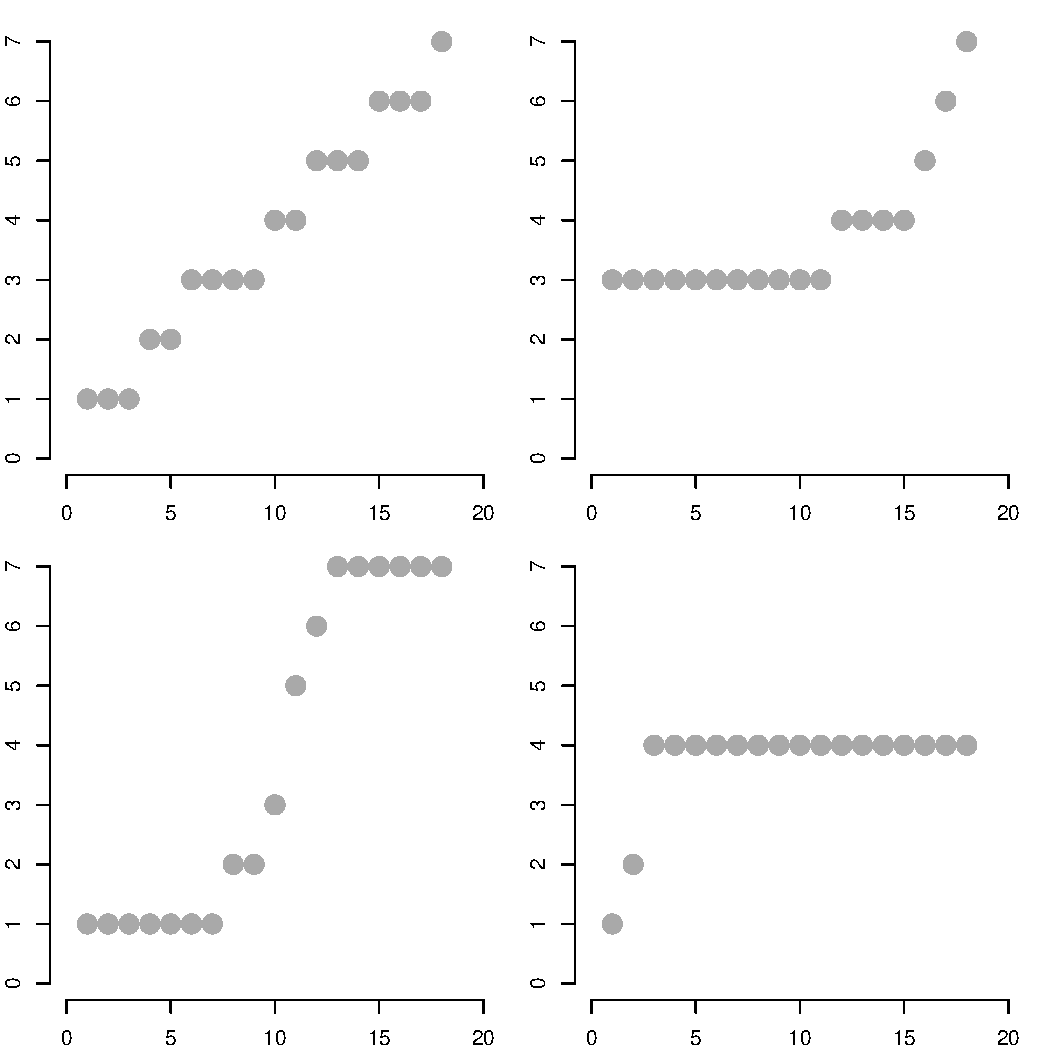
\includegraphics[height=0.75\textheight]{RVorlesung/foursamples}
  \end{center}
\end{frame}

\begin{frame}
  {Verteilungsformen}
  \alert{Histogramme} | Vier Stichproben mit \alert{$\bar{x}=3.72$} und \alert{$n=18$}\\
  \Viertelzeile
  \grau{Zum Beispiel 18 Bewertungen eines Probanden auf einer 7-Punkt-Skala}\\
  \begin{center}
    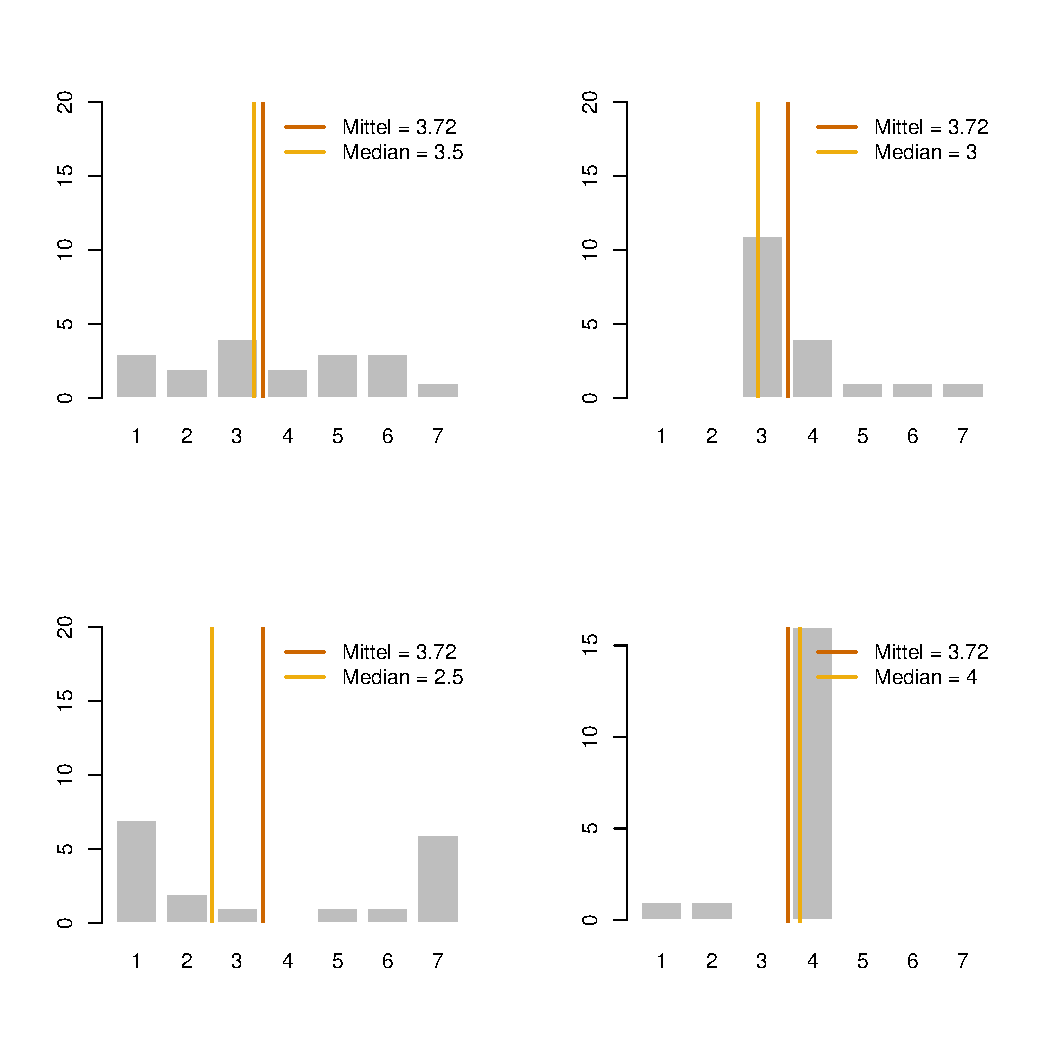
\includegraphics[height=0.75\textheight]{RVorlesung/fourdists}
  \end{center}
\end{frame}

\begin{frame}
  {Quartile}
  \alert{Quartile} | Generalisierung des Medians (bei 25 \%, 50 \%, 75 \%)\\
  \begin{center}
    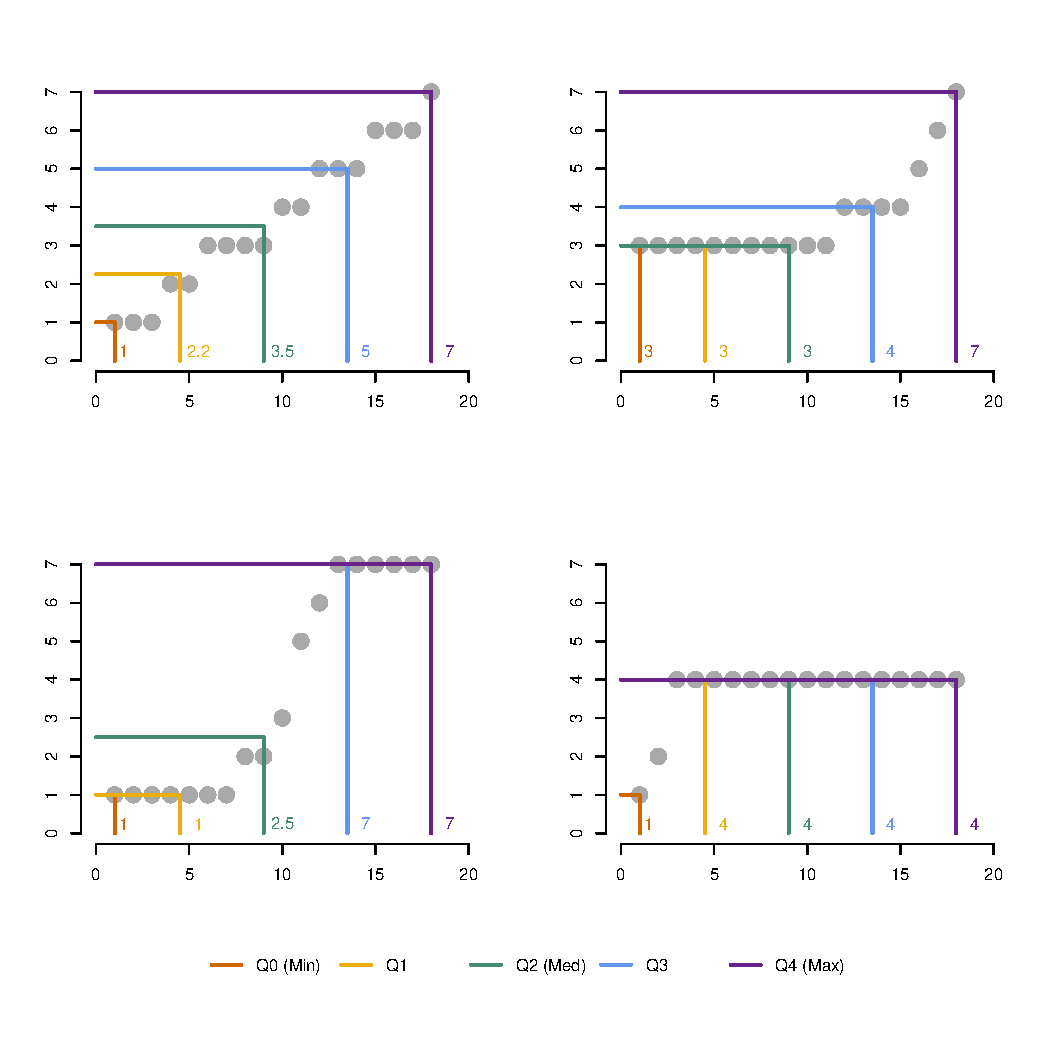
\includegraphics[height=0.85\textheight]{RVorlesung/fourquartiles}
  \end{center}
\end{frame}


\begin{frame}
  {Interquartilbereich, Boxplots und Violinplots}
  \begin{itemize}[<+->]
    \item Interquartilbereich \alert{$IQR = Q_3-Q_1$} | Die mittleren 50 \%
     \Zeile 
    \item Boxplots
      \Viertelzeile
      \begin{itemize}[<+->]
        \item \alert{Median} | Linie in der Mitte
        \item \alert{Oberes und unteres Quartil} | Boxen
        \item \alert{1,5-facher Interquartilabstand} | gestrichelte Hebel
        \item \alert{Ausreißer} | Punkte
      \end{itemize}
      \Halbzeile
    \item Violinplots | Zusätzlich Plot der Verteilungsdichte (statt Box)
  \end{itemize}
\end{frame}


\begin{frame}
  {Boxplots | Die bessere Zusammenfassung}
  \begin{center}
    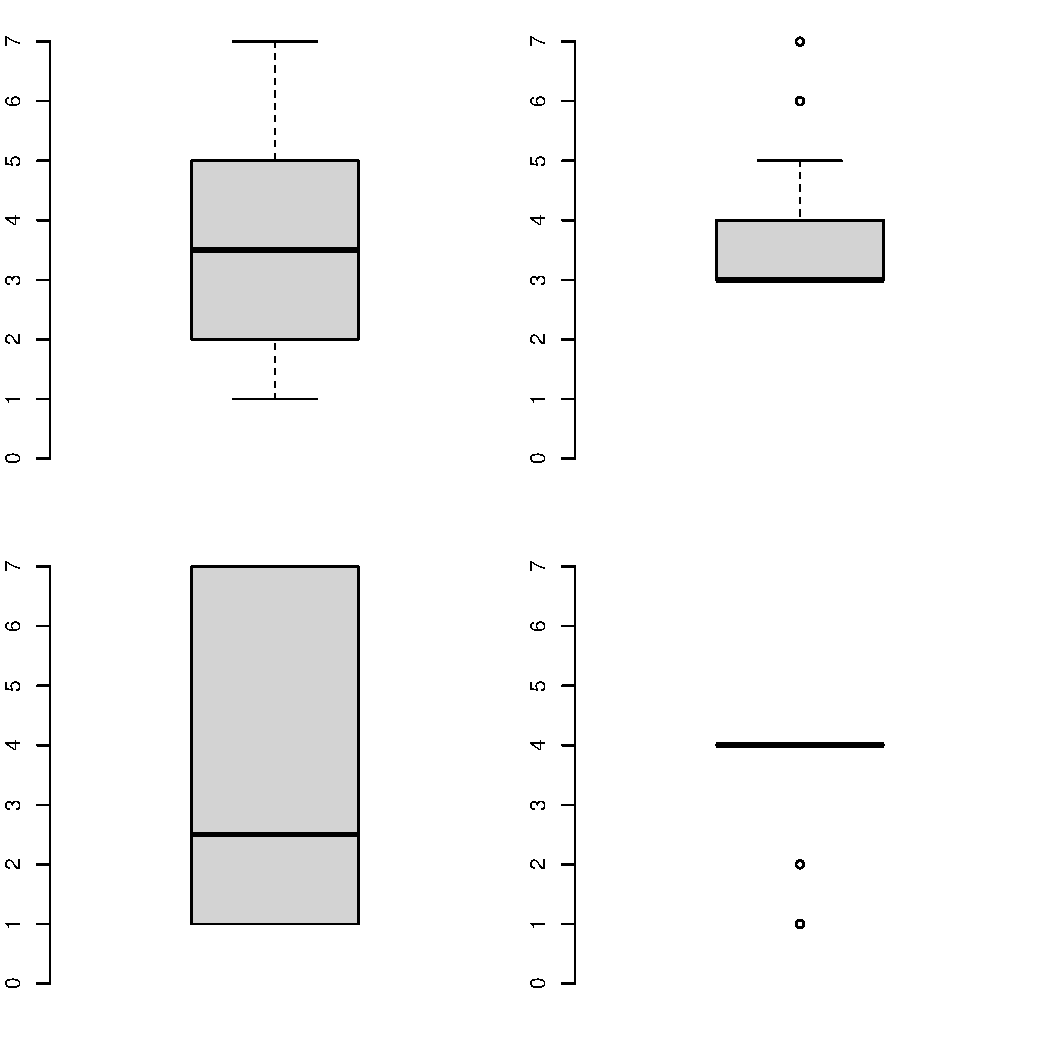
\includegraphics[height=0.7\textheight]{RVorlesung/fourbox}
  \end{center}
\end{frame}


\begin{frame}
  {Violinplots | Die noch bessere Zusammenfassung}
  \begin{center}
    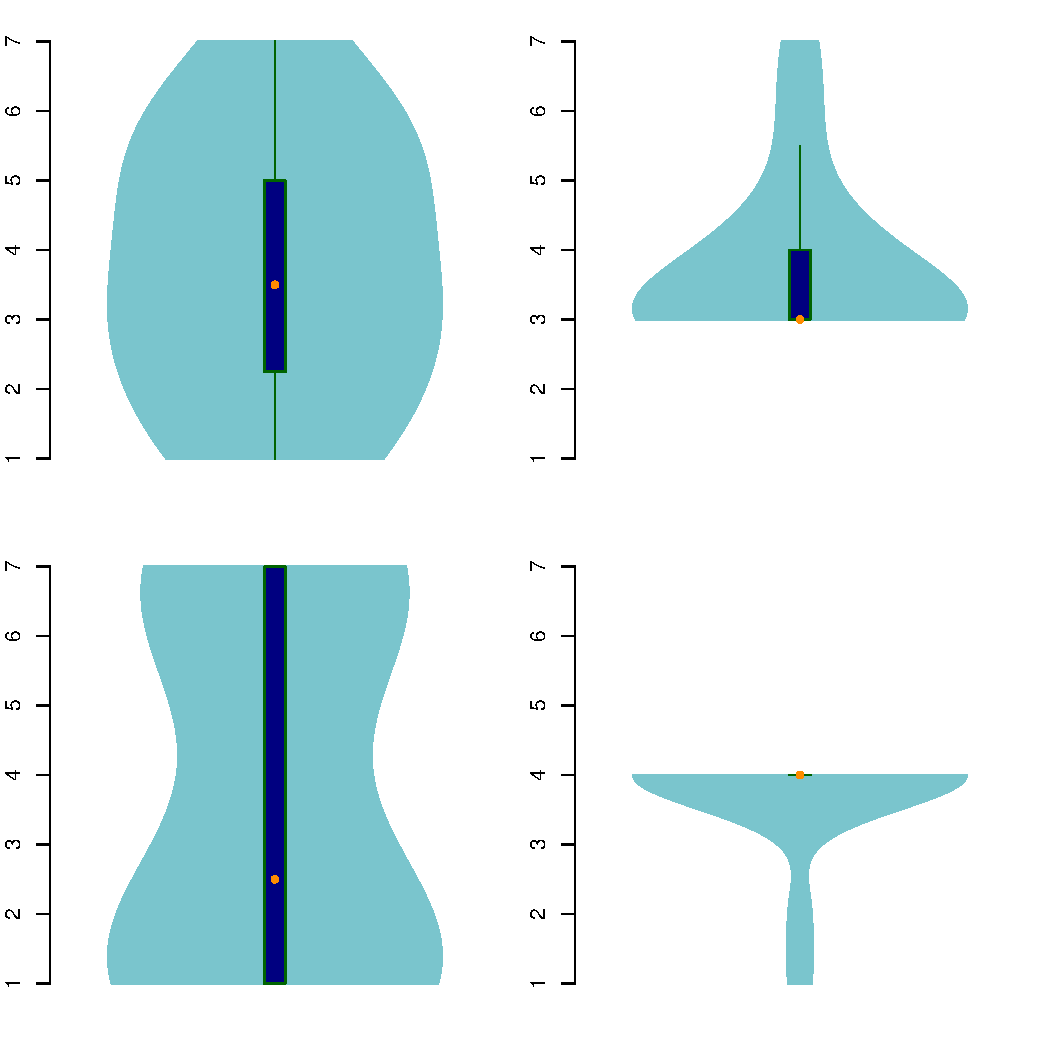
\includegraphics[height=0.7\textheight]{RVorlesung/fourviolins}
  \end{center}
\end{frame}

\begin{frame}
  {Was bestimmt die Varianz?}
  Die \alert{Distanzen der Messwerte zum Mittel} sind unterschiedlich groß.\\
  \begin{center}
    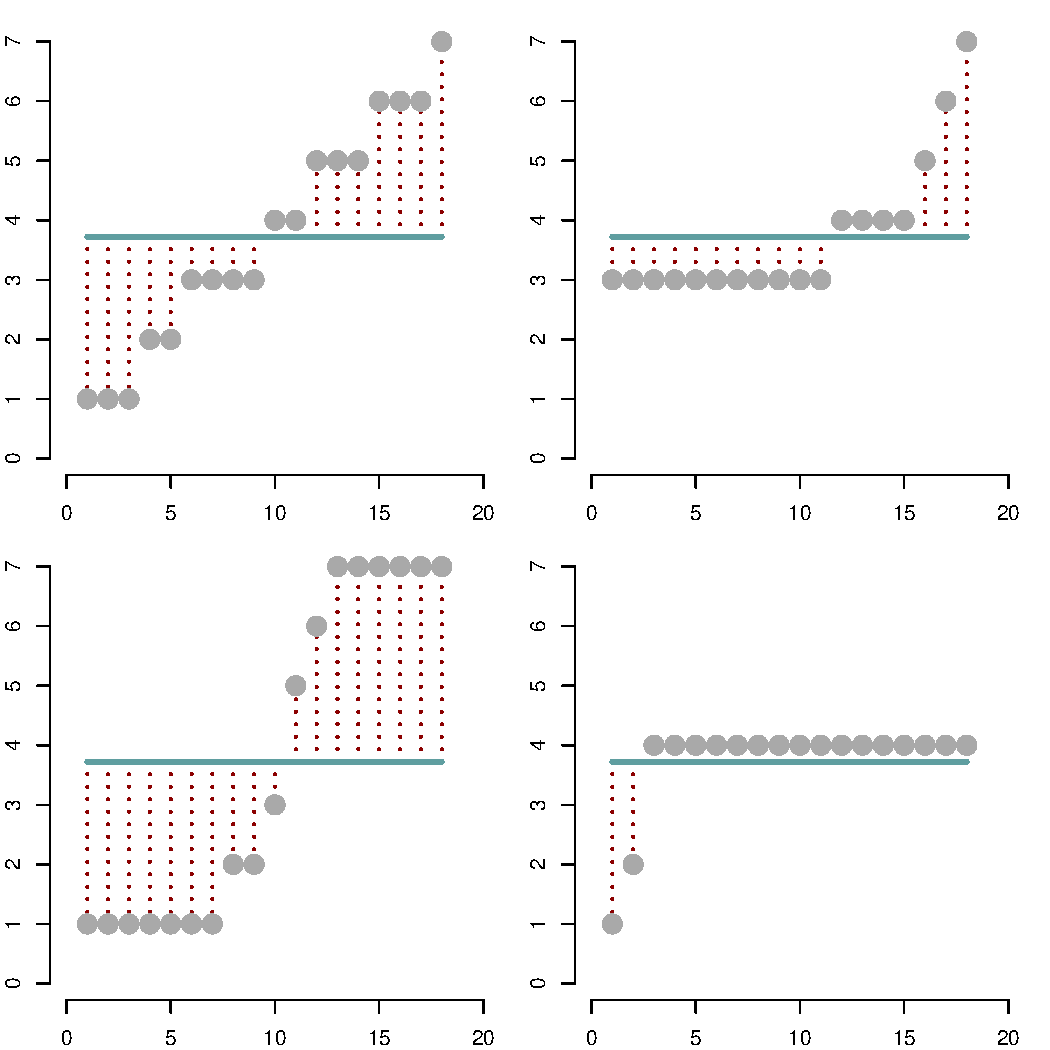
\includegraphics[height=0.7\textheight]{RVorlesung/fourvariances}
  \end{center}
\end{frame}


\begin{frame}
  {Varianz und Standardabweichung}
  \alert{Varianz $s^2$} | Quadrierte \alert{mittlere Abweichung} vom Mittelwert\\
      \begin{center}
	\alert{$s^2(x)=\frac{ \sum\limits_{i=1}^{n}(x_i-\bar{x})^2}{n-1}$}
      \end{center}
\pause
      \vspace{0.5cm}
    \alert{Standardabweichung $s$} | Quadratwurzel der Varianz\\
      \begin{center}
	\alert{$s(x)=\sqrt{s^2(x)}$}
      \end{center}
      \vspace{0.5cm}

  \pause
    \alert{Summe der Quadrate} | Zählerterm der Varianz\\
  \begin{center}
    $SQ(x)=\sum\limits_{i=1}^{n}(x_i-\bar{x})^2$
  \end{center}
\end{frame}

\begin{frame}
  {Unterschiedliche Standardabweichungen}
  \begin{center}
    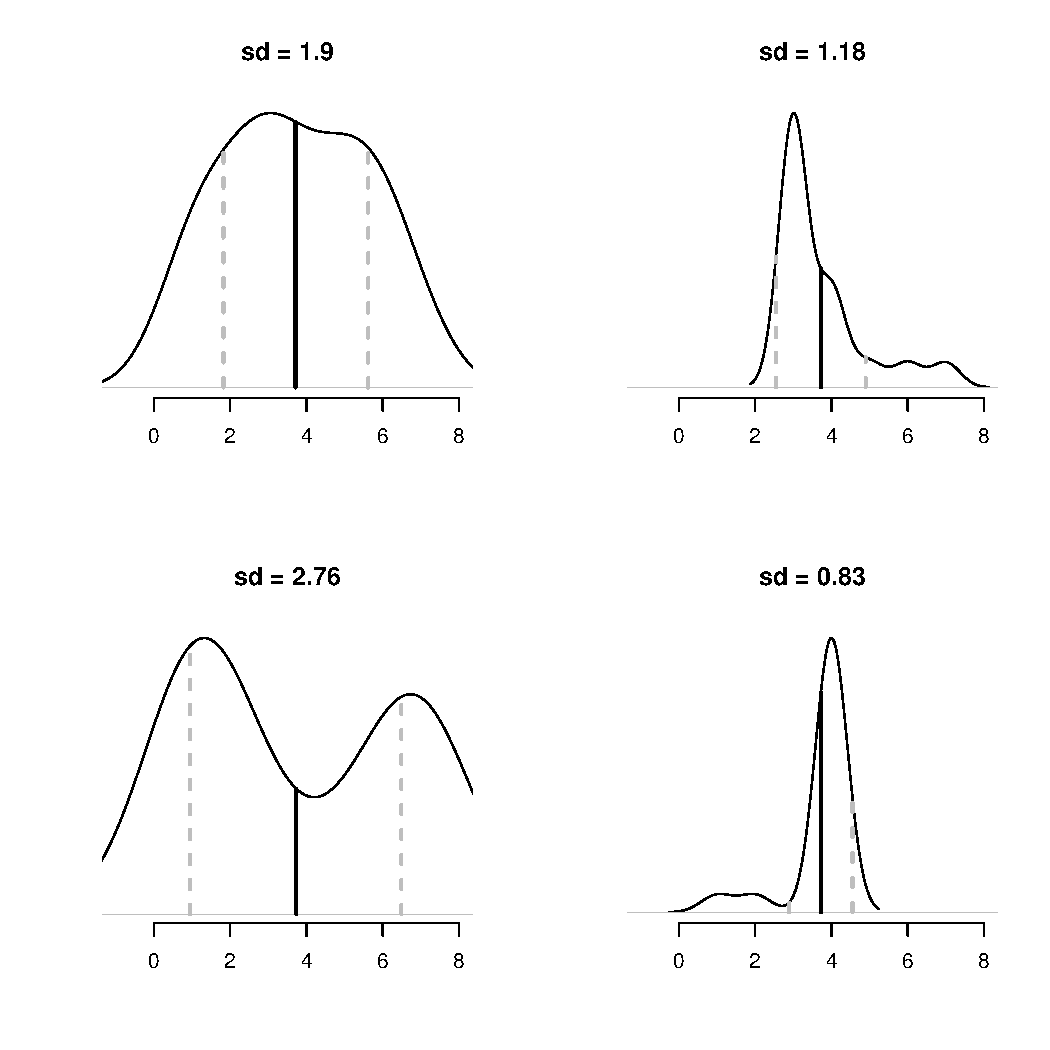
\includegraphics[height=0.9\textheight]{RVorlesung/stdevs}
  \end{center}
\end{frame}


\begin{frame}
  {z-Wert}
  Für jeden Messpunkt $x_i$ | \alert{$z_i=\frac{x_i-\bar{x}}{s(x)}$}\\
  \begin{center}
    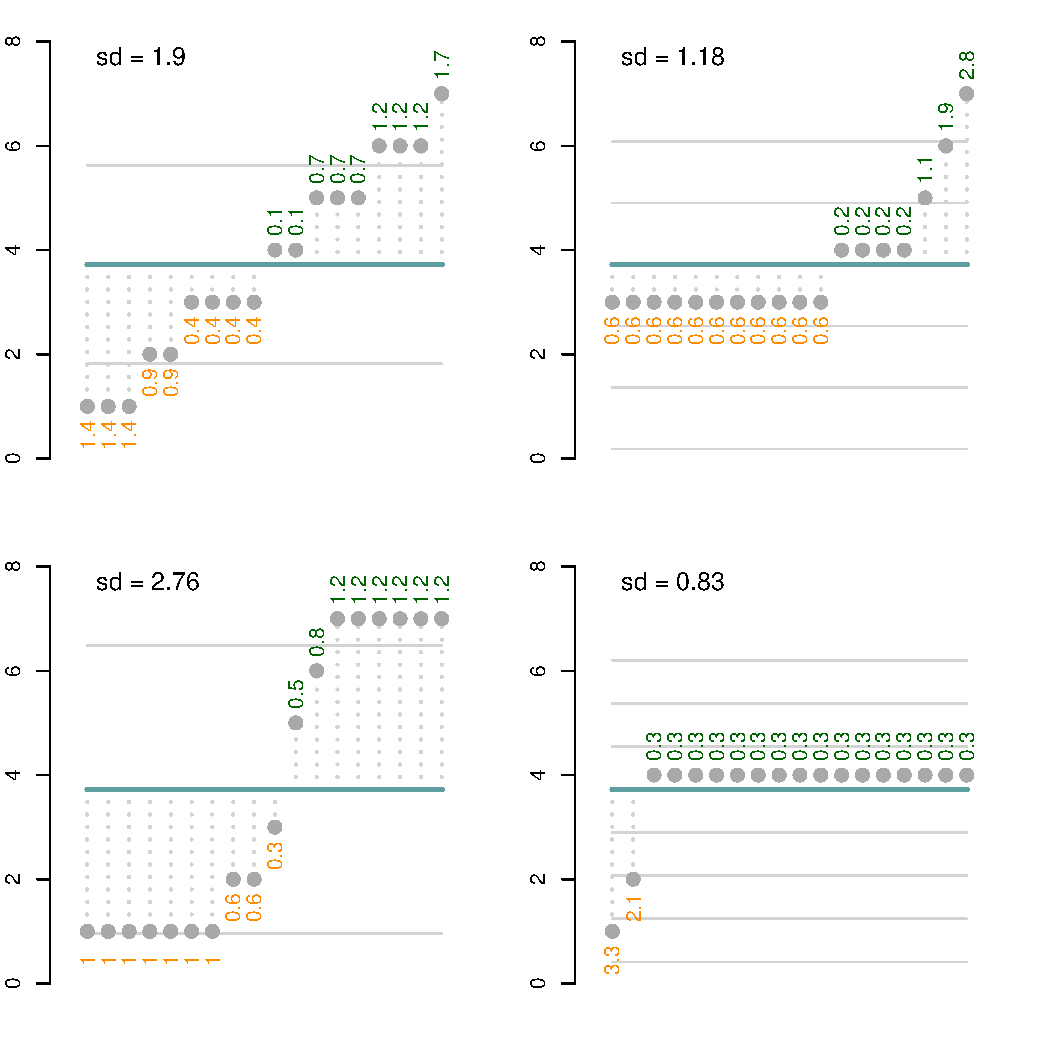
\includegraphics[height=0.8\textheight]{RVorlesung/fourzs}
  \end{center}
\end{frame}

\begin{frame}
  {z-Wert | Rechenbeispiel}
  \begin{itemize}[<+->]
    \item Bsp.: $\alert{x}=[3.9, 4.3, 7.2, 8.5, 11.1, 12.1, 14.0, 20.7]$
      \Halbzeile
      \begin{itemize}[<+->]
        \item $\alert{\bar{x}}=$\onslide<2->{$10.225$}
          \Halbzeile
        \item $\alert{s^2(x)}=$$\frac{(3.9-10.255)^2+\ldots+(20.7-10.225)^2}{8-1}=$$\frac{215.495}{7}=$$30.785$
          \Halbzeile
        \item $\alert{s(x)}=$$\sqrt{30.785}=$$5.548$
          \Halbzeile
        \item $\alert{z}=[\frac{3.9-10.225}{5.548}$, \ldots, $\frac{20.7-10.225}{5.548}]=$$[-1.140, -1.068, -0.545, -0.311, 0.158, 0.338, 0.680, 1.888]$
      \end{itemize}
  \end{itemize}
\end{frame}

\section{Bivariate Statistiken}

\begin{frame}
  {Zähldaten von zwei Variablen}
  \alert{Kreuztabelle} | Darstellung der Zähldaten zweier Variablen\\
  \Zeile
  \begin{center}
    \begin{tabular}{rcc}
      \cline{2-3}
      &&\\
      & \textbf{Variable 1 | Wert 1} & \textbf{Wert2} \\
      &&\\
      \hline
      &&\\
      \textbf{Variable 2 | Wert 1} & Anzahl $x_{11}$ & Anzahl $x_{12}$ \\
      &&\\
      \textbf{Wert 2} & Anzahl $x_{21}$ & Anzahl $x_{22}$ \\
      &&\\
      \hline
    \end{tabular}
  \end{center}
\end{frame}



\section{Standardfehler und Konfidenzintervalle}

\begin{frame}
  {Anteilswerte und Stichproben}
  \begin{itemize}[<+->]
    \item Das Verb \textit{essen} | Manchmal mit, manchmal ohne Akkusativ (direktes Objekt)
    \item Angenommenes wahres Verhältnis | \alert{Mit Objekt 39 \%, ohne Objekt 61 \%}
      \Halbzeile
    \item Viele Stichproben mit n=100 | Ergebnis \rot{nicht} immer 39 zu 61
     \Doppelzeile 
    \item \alert{95\%-Konfidenzintervall} \\
      \gruen{In welchem Bereich liegen 95\% aller Anteilswerte bei n=100?}
  \end{itemize}
\end{frame}


\begin{frame}
  {Sechzehn simulierte Stichprobenentnahmen (n=100)}
  \centering 
  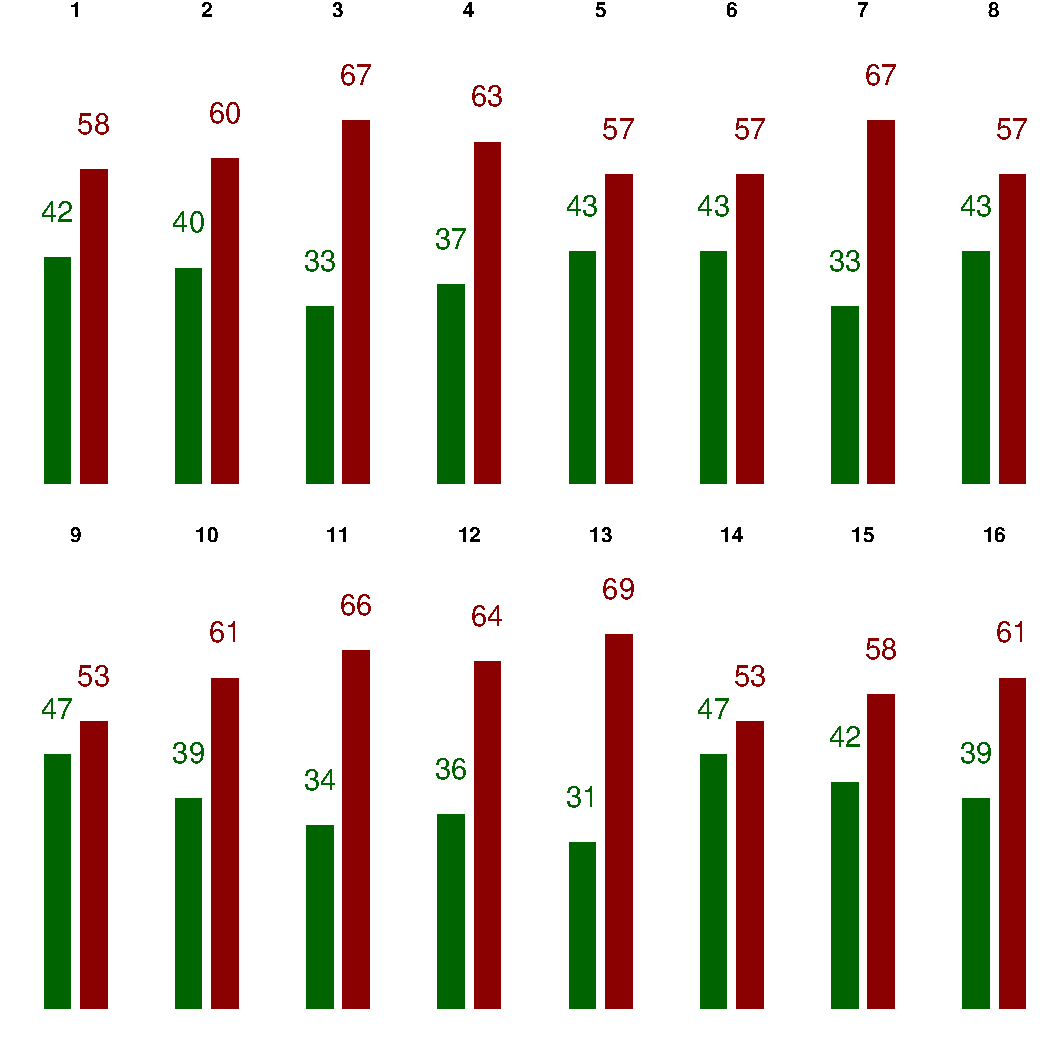
\includegraphics[height=0.8\textheight]{RVorlesung/sixteenbernoullis}
\end{frame}

\begin{frame}
  {Wiederholte Stichprobenentnahmen (n=100)}
  \centering 
  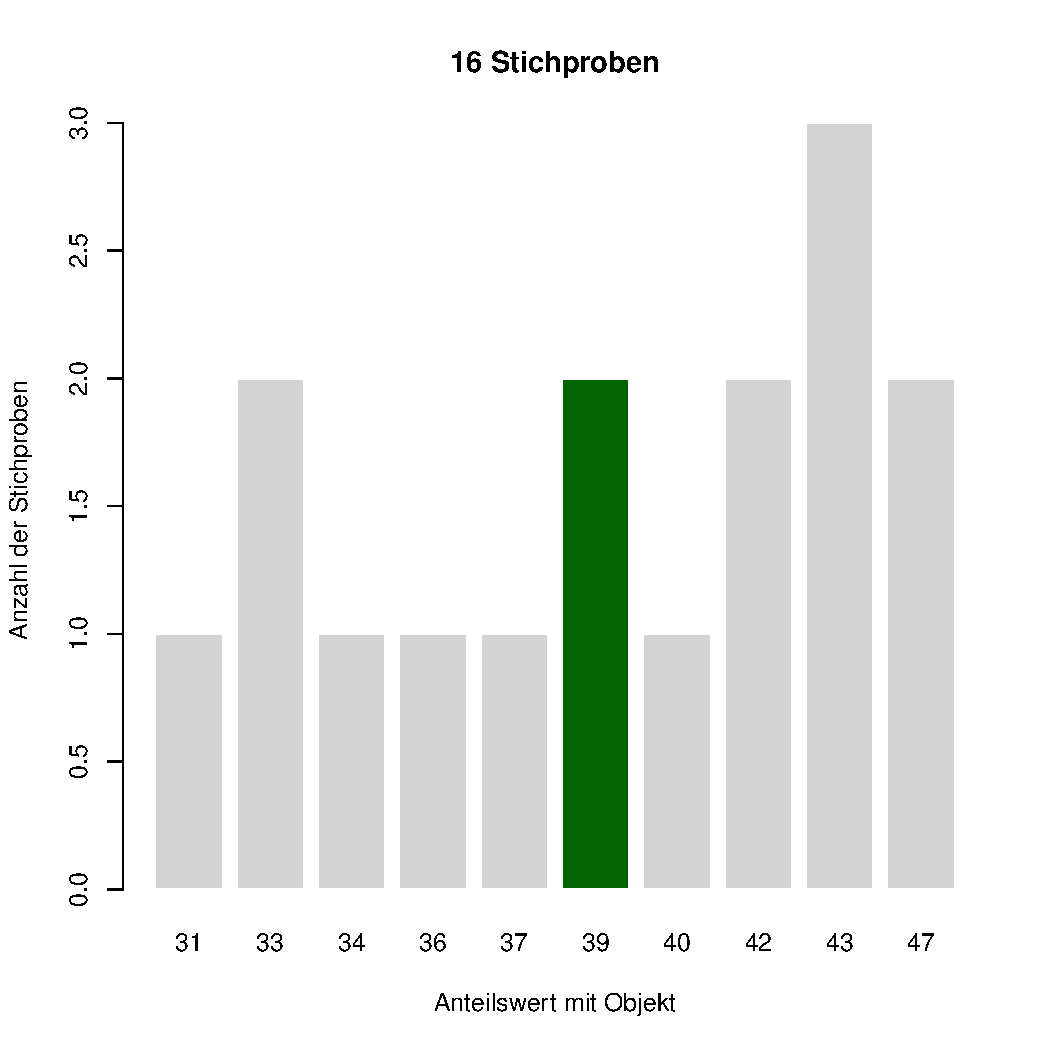
\includegraphics[width=0.3\textwidth]{RVorlesung/manybernoullis1}
  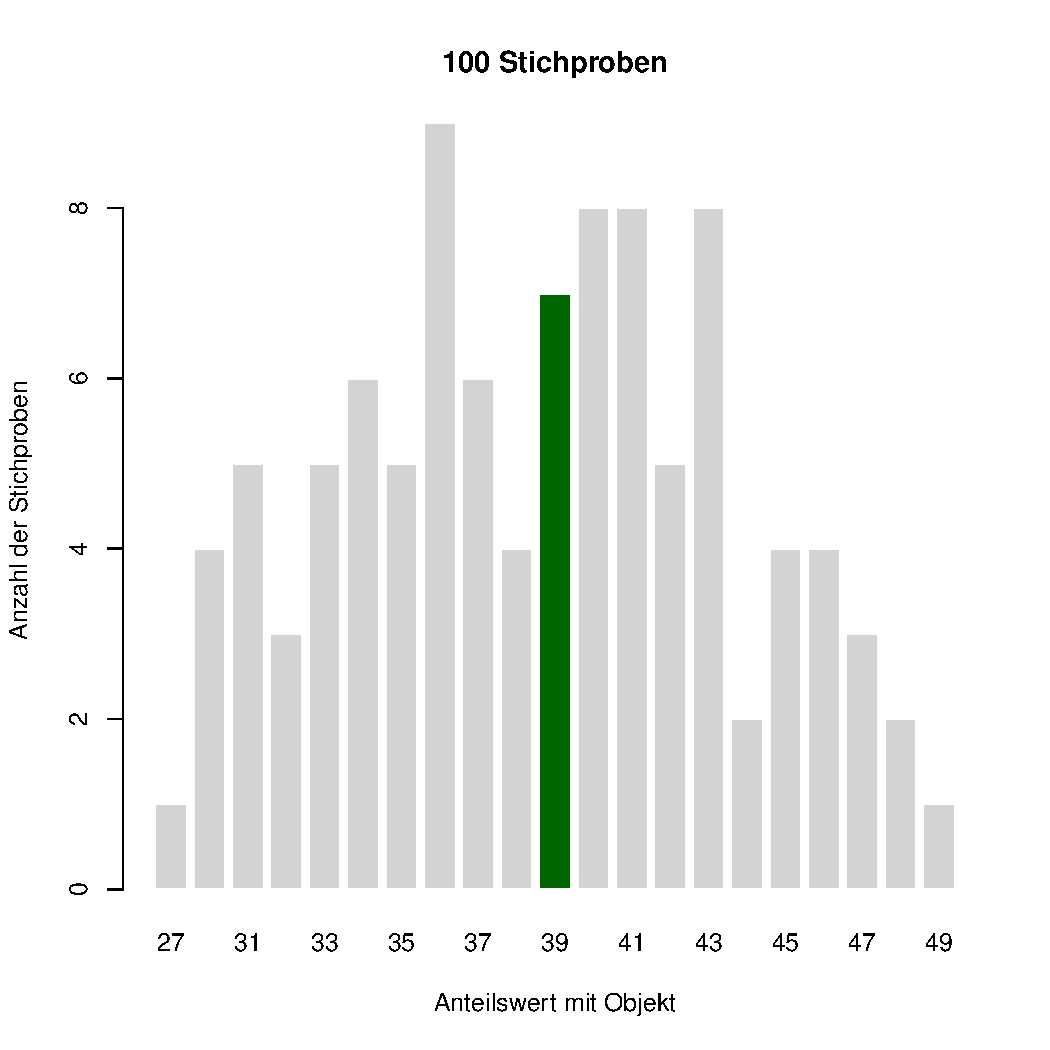
\includegraphics[width=0.3\textwidth]{RVorlesung/manybernoullis2}
  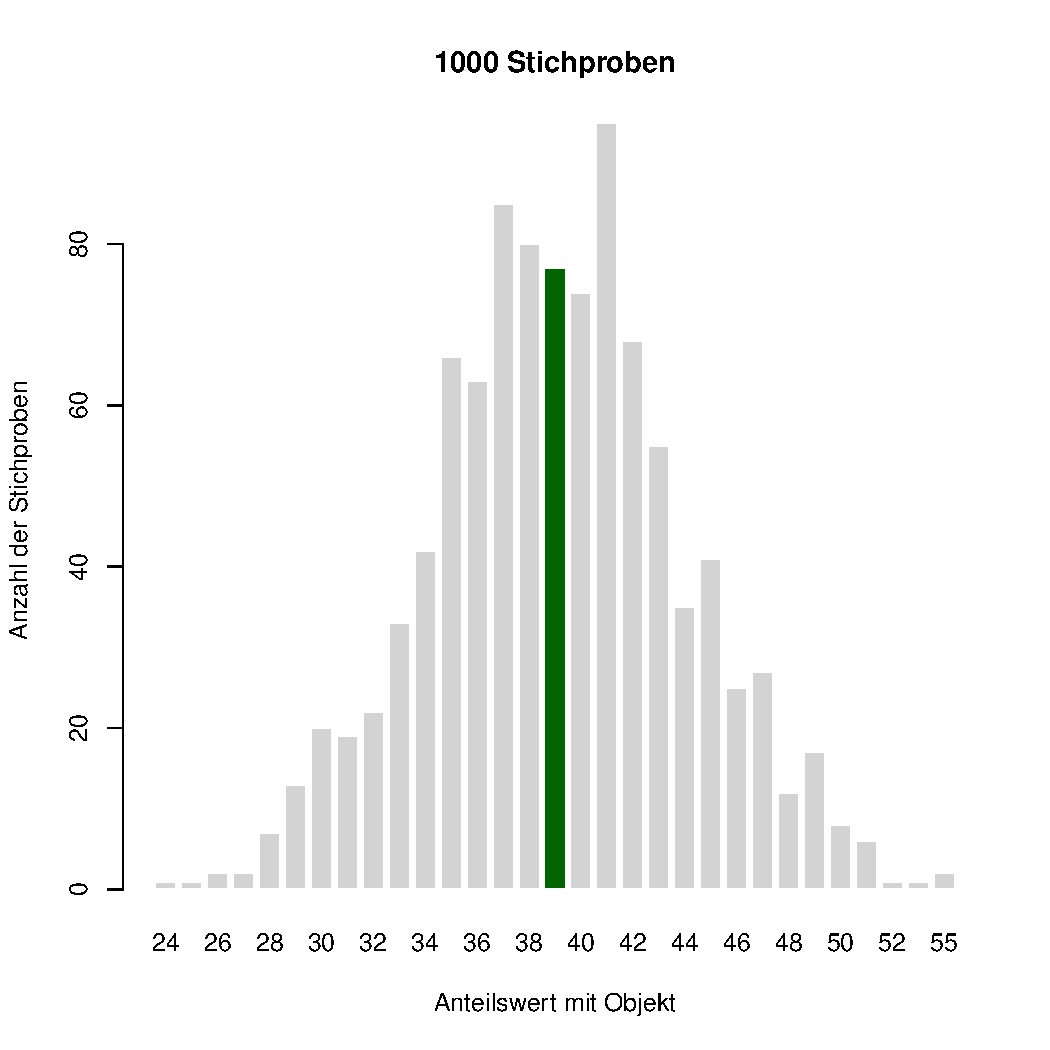
\includegraphics[width=0.3\textwidth]{RVorlesung/manybernoullis3}
\end{frame}


\begin{frame}
  {Standardfehler}
  \begin{itemize}[<+->]
    \item Die \alert{meisten $q$} | Nah am wahren Wert $Q$
    \item Sehr \alert{wenige $q$} | Weit von $Q$ entfernt
      \Halbzeile
    \item Bei unendlich vielen Messungen
      \begin{itemize}[<+->]
        \item \alert{\orongsch{Mittelwert} der gemessenen Anteilswerte gleich $Q$}
        \item Gemessene Anteilswerte \orongsch{normalverteilt um $Q$}
        \item \alert{Standardabweichung} der Messwerte um Q bekannt \ding{222} \gruen{Standardfehler}
      \end{itemize}
     \Zeile 
    \item \gruen{Standarfehler} | Standardabweichung der Messwerte
      \begin{itemize}[<+->]
        \item Bei \alert{gegebener Stichprobengröße $n$}
        \item Bei einem \alert{bekannten Populationsanteil Q}
      \end{itemize}
  \end{itemize}
\end{frame}

\begin{frame}
  {Standardfehler für Anteilswerte | Berechnung}
  \begin{itemize}[<+->]
    \item Für einen wahren Anteilswert $Q$
    \item Bei Stichprobengröße $n$
  \end{itemize}
  \Halbzeile
  \begin{center}
    \alert{$SF(Q,n)=\sqrt{\frac{Q\cdot(1-Q)}{n}}$}\\
    \Doppelzeile
    Bsp. für $Q=0.39$ und $n=100$ | $SF(q)=\sqrt{\frac{0.39\cdot(1-0.39)}{100}}=0.0488$
  \end{center}
\end{frame}

\begin{frame}
  {Standardfehler | Interpretation}
  \begin{center}
    \alert{$SF(Q,n)=\sqrt{\frac{Q\cdot(1-Q)}{n}}$}\\

    \vspace{.1cm}
    Bsp.: $SF(0.39,100)=\sqrt{\frac{0.39\cdot(1-0.39)}{100}}=0.0488$
  \end{center}
  \Zeile
  \begin{itemize}[<+->]
    \item Für \alert{beliebig viele} Stichproben
    \item Bei \alert{Stichprobengröße $n=100$}
    \item Aus einer Grundgesamtheit mit \alert{wahrem Anteilswert $Q=0.39$}
      \Halbzeile
    \item Abweichung der gemessenen Anteile von $Q=0.39$ mit einem \alert{$SF=0.0488$}
  \end{itemize}
\end{frame}


\begin{frame}
  {Konfidenzintervall | Standardfehler und Normalverteilung}
  \alert{Normal-\slash Gaussverteilung} | Parameter \alert{Mittelwert} und \alert{Standardabweichung}\\
  \Viertelzeile
  \ding{222} Mathematisch exhaustiv bekannt, Flächen unter der Kurve usw.\ berechenbar\\
  \centering
  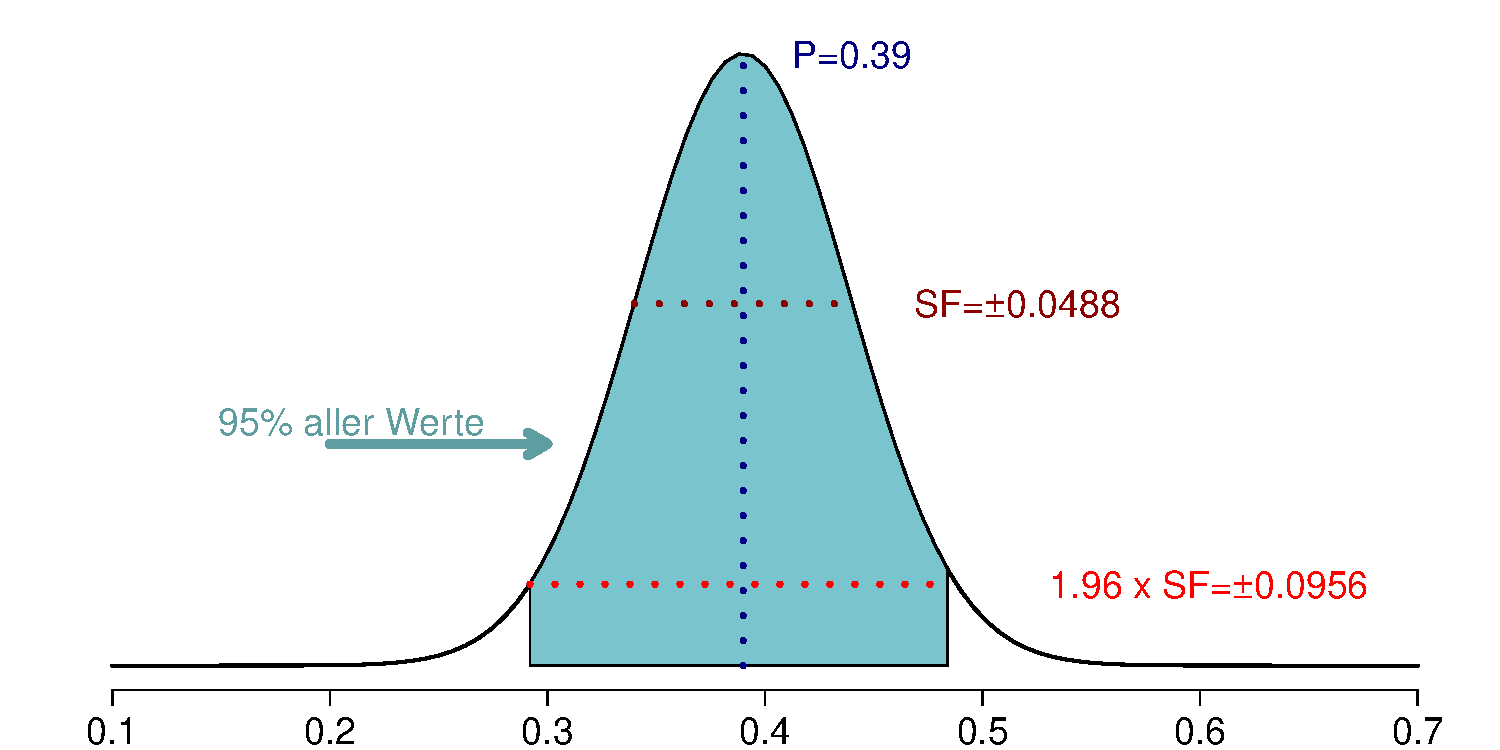
\includegraphics[height=0.75\textheight]{RVorlesung/ci95}
\end{frame}


\begin{frame}
  {Verteilungsfunktion der Normalverteilung}
  \onslide<+->
  \onslide<+->
  \centering 
  \LARGE
  \begin{math}
    p(\orongsch{x})=\grau{\frac{1}{\gruen{\sigma}\sqrt{2\pi}}}e^{-\frac{1}{2}\left(\frac{\orongsch{x}-\alert{\mu}}{\gruen{\sigma}}\right)^2}
  \end{math}\\
  \large
  \Doppelzeile
  Wenn Sie mehr wissen möchten:\\
  \url{https://youtu.be/cy8r7WSuT1I}\\
  Großartiges Video von Grant Sanderson (3blue1brown)
\end{frame}


\begin{frame}
  {Konfidenzintervall | z-Werte}
  \begin{itemize}[<+->]
    \item Stichproben (wie erwähnt) \alert{normalverteilt} 
    \item Der \alert{z-Wert}, zum Beispiel für $\alpha=0.95$: \alert{$z(0.95)$} beantwortet:\\
      \orongsch{Wie viele Standardfehler definieren 95\% der Fläche unter der Kurve?}
      \Zeile
    \item \alert{Quantilfunktion der Normalverteilung} | In R mit \alert{\texttt{qnorm()}} oder \alert{Tabelle}
    \item Quantilfunktion | Wie viele Standardabweichungen trennen auf jeder Seite 2.5\% ab?
    \item \alert{\texttt{qnorm(0.025, lower.tail=FALSE)}} \ding{222} \orongsch{$z(0.95) = 1.96$}
  \end{itemize}
\end{frame}

\begin{frame}
  {Konfidenzintervall | Standardfehler um wahren Anteilswert}
  \begin{itemize}[<+->]
    \item Standardfehler | \alert{Standardabweichung} der Stichprobenwerte
    \item \alert{Konfidenzbreite} | \orongsch{z-Wert multipliziert mit Standardfehler}
    \item 95\% der Werte | Intervall \orongsch{Anteilswert ± Konfidenzbreite}
  \end{itemize}
  \Doppelzeile
  \begin{center}
    \alert{$KI(Q,n,\alpha)=Q\pm z(\alpha)\cdot SF(Q,n)$}\\
    \Zeile
  Bsp.: $KI(0.39,100,0.95)=0.39\pm1.96\cdot 0.0488=0.39\pm0.096=\alert{[0.29, 0.49]}$
  \end{center}
\end{frame}

\begin{frame}
  {Interpretation}
  \begin{center}
    Konfidenzintervall im Beispiel | \alert{0.29 bis 0.49}\\
    \Halbzeile
    In 95\% aller Stichproben mit $n=100$ liegt der Messwert\\
    zwischen $0.29$ und $0.49$ bei einem wahren Anteil von 0.39.
  \end{center}
  \Zeile
  \begin{itemize}[<+->]
    \item Praxis | \orongsch{Wahrer Anteil nicht bekannt}, daher \orongsch{Schätzung aus Stichprobenanteil $q$}
    \Zeile
    \item \rot{Der gemessene Anteil $q$ kann aber eine totale Fehlschätzung sein!}
    \item Die Philosophie dahinter geht von \alert{wiederholten Messungen} aus.
      \Halbzeile
    \item Entweder liegt der gemessene Wert im Konfidenzintervall,\\
      \rot{oder ein seltenes Ereignis ist eingetreten}.
      \Halbzeile
    \item \rot{\textbf{Falsche Interpretation}:\\Wir sind zu 95\% sicher, dass der wahre Wert zwischen 0.29 und 0.49 liegt.}
  \end{itemize}
\end{frame}

\begin{frame}
  {Konfidenzintervall | Breite bei verschiedenen Q, n und $\alpha$}
  \centering 
  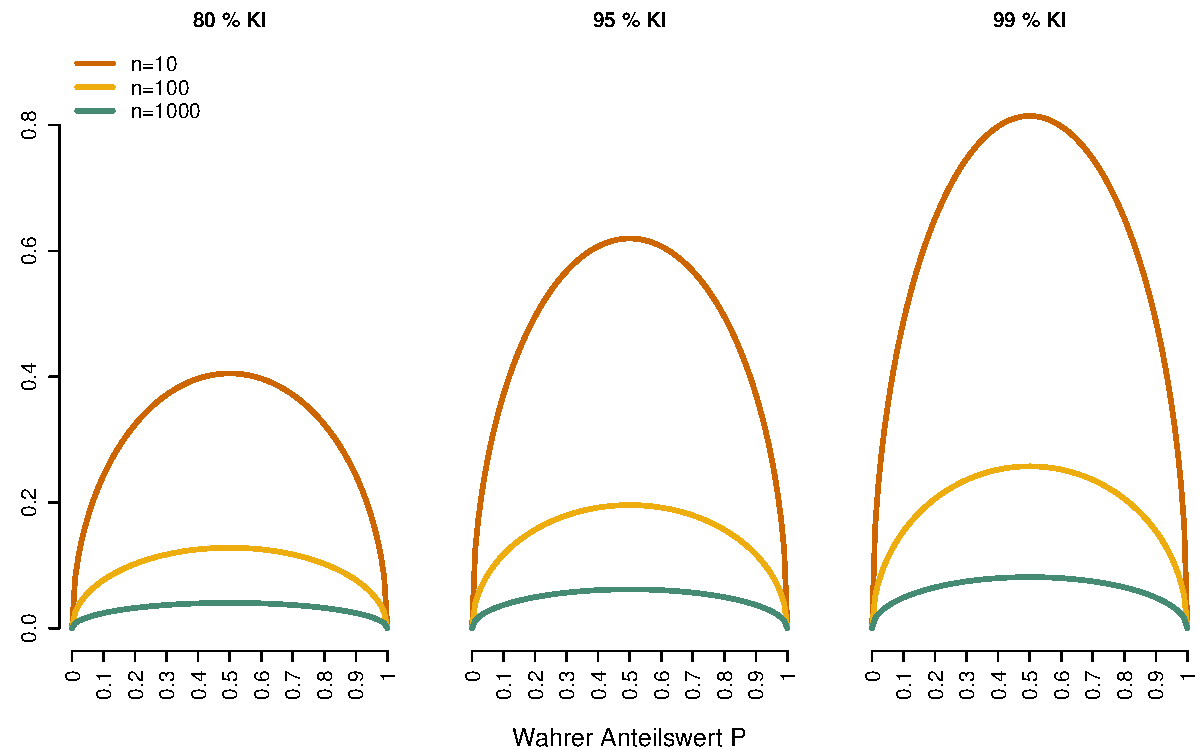
\includegraphics[height=0.85\textheight]{RVorlesung/threecis}
\end{frame}

\begin{frame}
  {Konfidenzintervall für Mittelwerte}
  \onslide<+->
  \onslide<+->
  Parallel zum KI für Anteilswerte: \alert{KI für Mittelwerte} mit \orongsch{derselben Formel}\\
  \Doppelzeile
  \onslide<+->
  \centering 
  Nur der Standardfehler wird anders berechnet:\\
  \Zeile
  \alert{$SF(\sigma, n)=\frac{\sigma}{\sqrt(n)}$}\\
  \Halbzeile
  \grau{$KI(\bar{x},n,\alpha)=\bar{x}\pm z(\alpha)\cdot SF(\sigma,n)$}\\
  \onslide<+->
  \Doppelzeile
  Interpretation des KI (95\%): Für einen \alert{beliebigen Mittelwert $\bar{x}$}\\
  und die \alert{wahre Standardabweichung der Population $\sigma$} liegen\\
  im Grenzwert exakt \alert{95\% aller Stichproben der Größe $n$ im 95\%-KI}.\\
  \Zeile
  Hier wird die wahre Standardabweichung $\sigma$ ggf.\\
  aus der Standardabweichung $s(x)$ Stichprobe geschätzt.
\end{frame}

\begin{frame}
  {Zur Interpretation des KIs}
  \onslide<+->
  \onslide<+->
  \centering 
  Schauen Sie sich möglichst mein (sehr altes) Video zur Interpretation von KIs an,\\
  auch wenn ich deutlich weniger im Kopf habe als Grant Sanderson.\\
  \Zeile
  \url{https://www.youtube.com/watch?v=TG8Z3RXL4E8X}
\end{frame}


\begin{frame}
  {Kritische Werte für Normalverteilung}
  \centering 
  \begin{tabular}[h]{ccp{0.1\textwidth}cc}
    \toprule
    \textbf{$\alpha$} & \textbf{$z(\alpha)$} && \textbf{$\alpha$} & \textbf{$z(\alpha)$}\\
    \midrule
    0.99 & 2.576 && 0.84 &  1.405 \\
    0.98 & 2.326 && 0.83 &  1.372 \\
    0.97 & 2.170 && 0.82 &  1.341 \\
    0.96 & 2.054 && 0.81 &  1.311 \\
    0.95 & 1.960 && 0.80 &  1.282 \\
    0.94 & 1.881 && 0.79 &  1.254 \\
    0.93 & 1.812 && 0.78 &  1.227 \\
    0.92 & 1.751 && 0.77 &  1.200 \\
    0.91 & 1.695 && 0.76 &  1.175 \\
    0.90 & 1.645 && 0.75 &  1.150 \\
    0.89 & 1.598 && & \\ 
    0.88 & 1.555 && & \\ 
    0.87 & 1.514 && & \\ 
    0.86 & 1.476 && & \\ 
    0.85 & 1.440 && & \\ 
    \bottomrule
  \end{tabular}
\end{frame}

\ifdefined\TITLE
  \section{Nächste Woche | Überblick}

  \begin{frame}
    {Einzelthemen}
    \begin{enumerate}
      \item Inferenz
      \item Deskriptive Statistik
      \item \alert{Nichtparametrische Verfahren}
      \item z-Test und t-Test
      \item ANOVA
      \item Freiheitsgrade und Effektstärken
      \item Power und Severity
      \item Lineare Modelle
      \item Generalisierte Lineare Modelle
      \item Gemischte Modelle
    \end{enumerate}
  \end{frame}
\fi
